Hubo2 Plus, Hubo for short, is a 130 $cm$ (4' 3'') tall, 42 $kg$ (93 $lb$) full-size humanoid robot.  
It was designed and constructed by Prof Jun-Ho Oh and the Hubo Lab at the Korean Advanced Institute of Science and Technology\cite{hubo-first}.
Hubo has 2 arms, 2 legs and a head, making it anthropomorphic to a human.  
It boasts 38 degrees of freedom (DOF) consisting of 6x in each leg, 6x in each arm, 5x in each hand, 3x in the neck, and 1x in the waist.
All joints with the exception of the fingers are high gain PD position controlled.
The fingers are PWM controlled.
It has a three axis force torque (FT) sensor on leg between the end of the ankle and the foot and on the arm where it connects to the hand.
Additionally it has accelerometers on each foot and a six axis inertial measurement unit (IMU) slightly below it's weight (approximately the centre of mass).
The reference commands for all of the joints are sent from the primary control computer (x86) to the individual motor controllers via two Controller Area Network (CAN) buses.
There are currently eight Hubo's functioning in the United States as of December 2012.
Four reside at Drexel University and one at Georgia Tech, Perdue, Ohio State and MIT.
Jaemi Hubo is the oldest of the Hubos in America and has been at the Drexel Autonomous Systems Lab\footnote{Drexel Autonomous Systems Lab: http://dasl.mem.drexel.edu/} (DASL) since 2008\cite{jaemiHuboSRM}.
Fig.~\ref{fig:hubo} shows the major dimensions of Hubo.

\begin{figure}[thpb]
  \centering
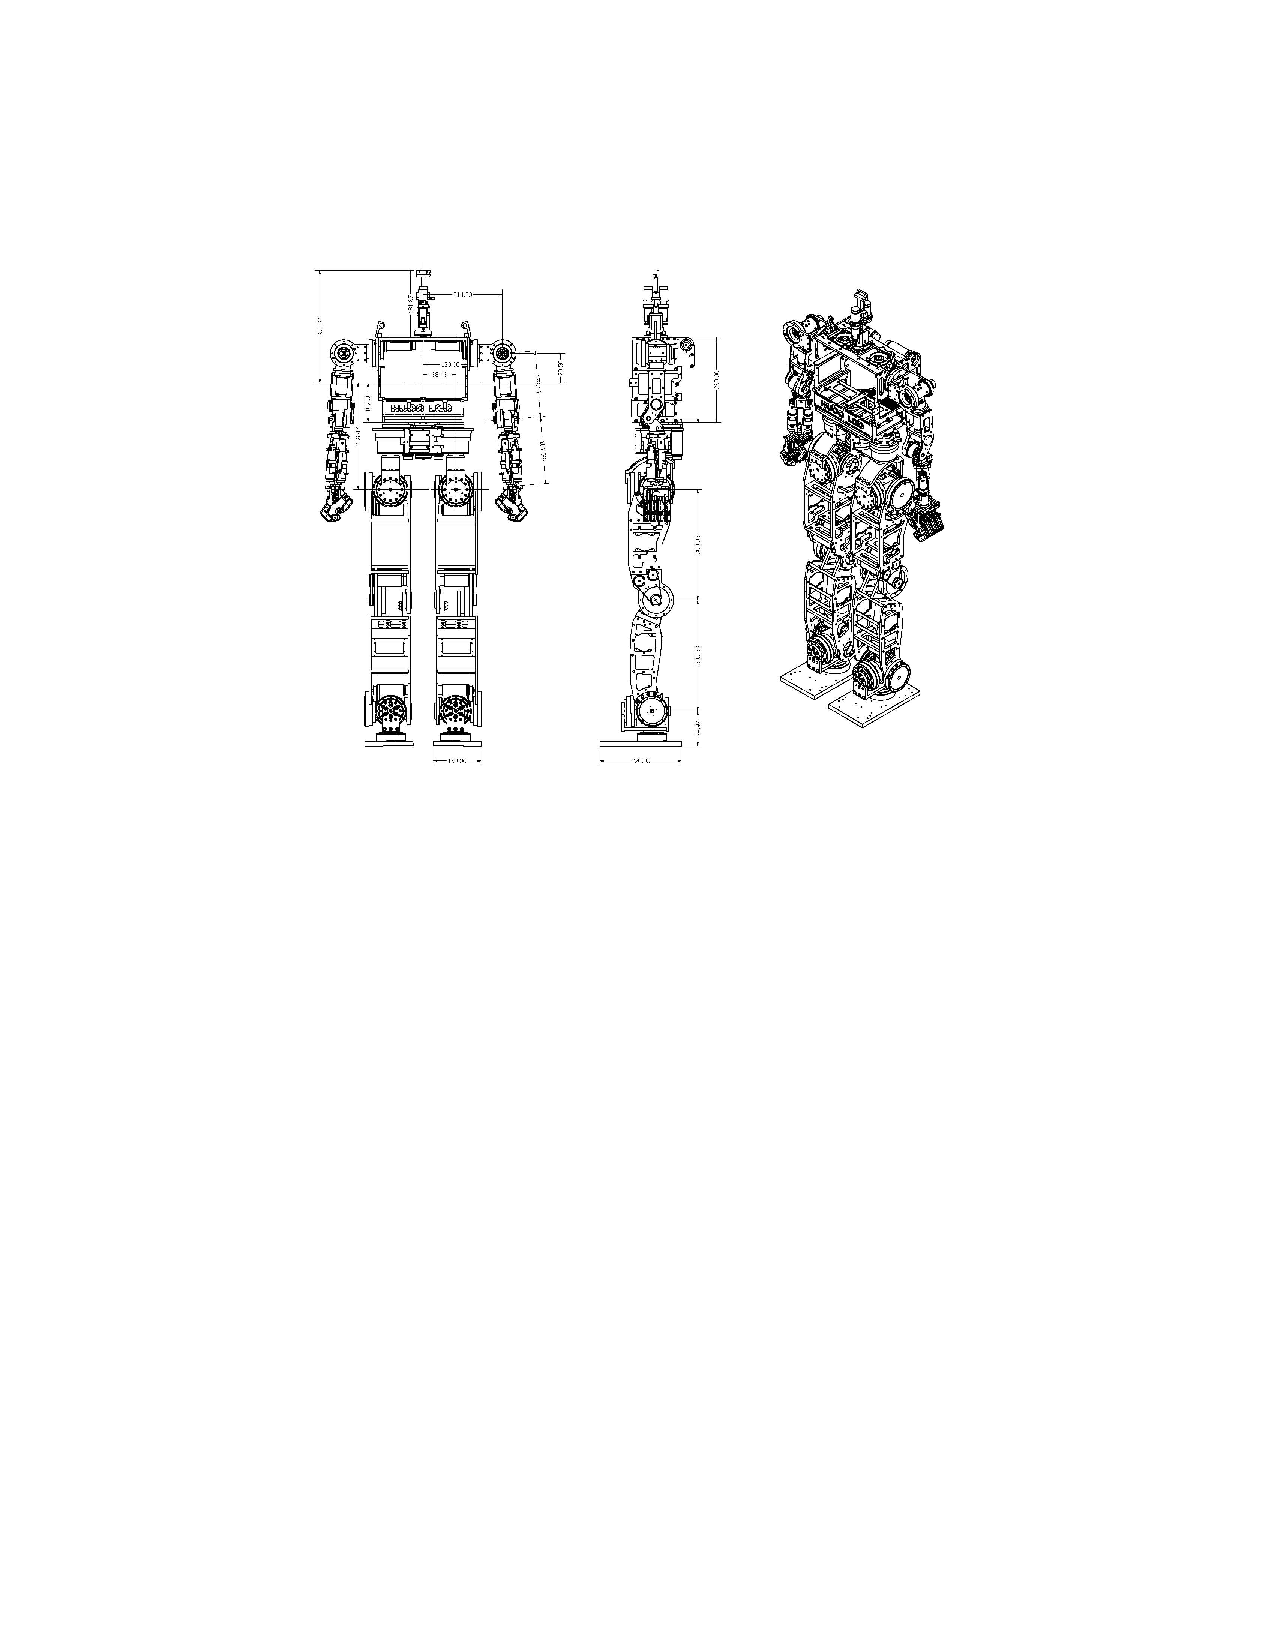
\includegraphics[width=1.0\columnwidth]{./pix/huboSkel.pdf}
  \caption{Hubo2 platform: 130 $cm$ tall full-size humanoid robot weighing 37 $kg$.  It has 38 DOF consisting of 6x in each leg, 6x in each arm, 5x in each hand, 1x in the waist, and 3x in the neck.}
  \label{fig:hubo}
\end{figure}

Hubo now runs on the Linux based, open-source, BSD licensed, system called Hubo-Ach.  
The overarching goal of the Hubo-Ach system is to create an easy to use interface between the Hubo hardware and the software environment.  
All system design decisions are made with the users, programmers and developers of the Hubo in mind.
This design philosophy streamlines closed-loop controller implementation, human robot interaction development and the utilization of popular robot related systems such as ROS\footnote{ROS: http://www.ros.org/} (Robot Operating System), OpenRAVE\footnote{OpenRAVE: http://openrave.org/} and MATLAB\footnote{MATLAB: http://www.mathworks.com/} on the Hubo platform.
Hubo-Ach also needs to be inherently robust because it is one of the software platforms being used by the DRC-Hubo\footnote{DRC-Hubo: http://drc-hubo.com/} DARPA Robot Challenge team where DASL is leading over half a dozen university labs.

Thus Hubo-Ach has great advantages over the Windows based software traditionally run on Hubo.
Hubo is traditionally run on software based in Windows utilizing the Real-Time framework called Real-Time Extensions (RTX) for Windows.
This software includes walking and other canned gestures with a user-friendly GUI making it a good choice for public demonstrations.
The overall system design is not conducive to adding additional closed-loop controllers, additional functionality or integration with third-party tools thus creating a critical-gap that must be crossed for increased software and controller development.
Hubo-Ach fills this critical-gap.


Hubo-Ach is the brain child of Daniel M. Lofaro\footnote{Daniel M. Lofaro: http://danlofaro.com/} of DASL at Drexel University in collaboration with \textit{Golems - The Humanoid Robotics Laboratory}\footnote{Golems - The Humanoid Robotics Labatory: www.golems.org/} at the Georgia Institute of Technology.  
The structure of Hubo-Ach can be seen in Fig.~\ref{fig:graph}.
Hubo-Ach runs in the background taking care of all CAN communications between the sensors/motor and the Hubo-Ach system.
Each of the Hubo's motor controllers uses a phase lock loop (PLL) to lock onto the reference update rate $f_r$ and perform linear interpolation between each reference command.  
The resulting motor controller command frequency $f_m$ is equal to five times $f_r$.
This reduces the jerk applied to each joint.
In order for the PLL to work effectively Hubo-Ach must sets the references for each joint at the real-time rate of $f_r$.
The sensors data is also received at the real-time rate of $f_r$.
Hubo-Ach is currently run at a $f_r$ of 200 $Hz$ utilizing approximately 78\% of the bandwidth on the CAN bus.

Hubo-Ach 
All of the reference and sensor data is set and made available to the user in $SI$ units by Hubo-Ach.

In order to keep the system 

It uses Ach as the primary IPC for communication between 




\begin{figure}[thpb]
  \centering
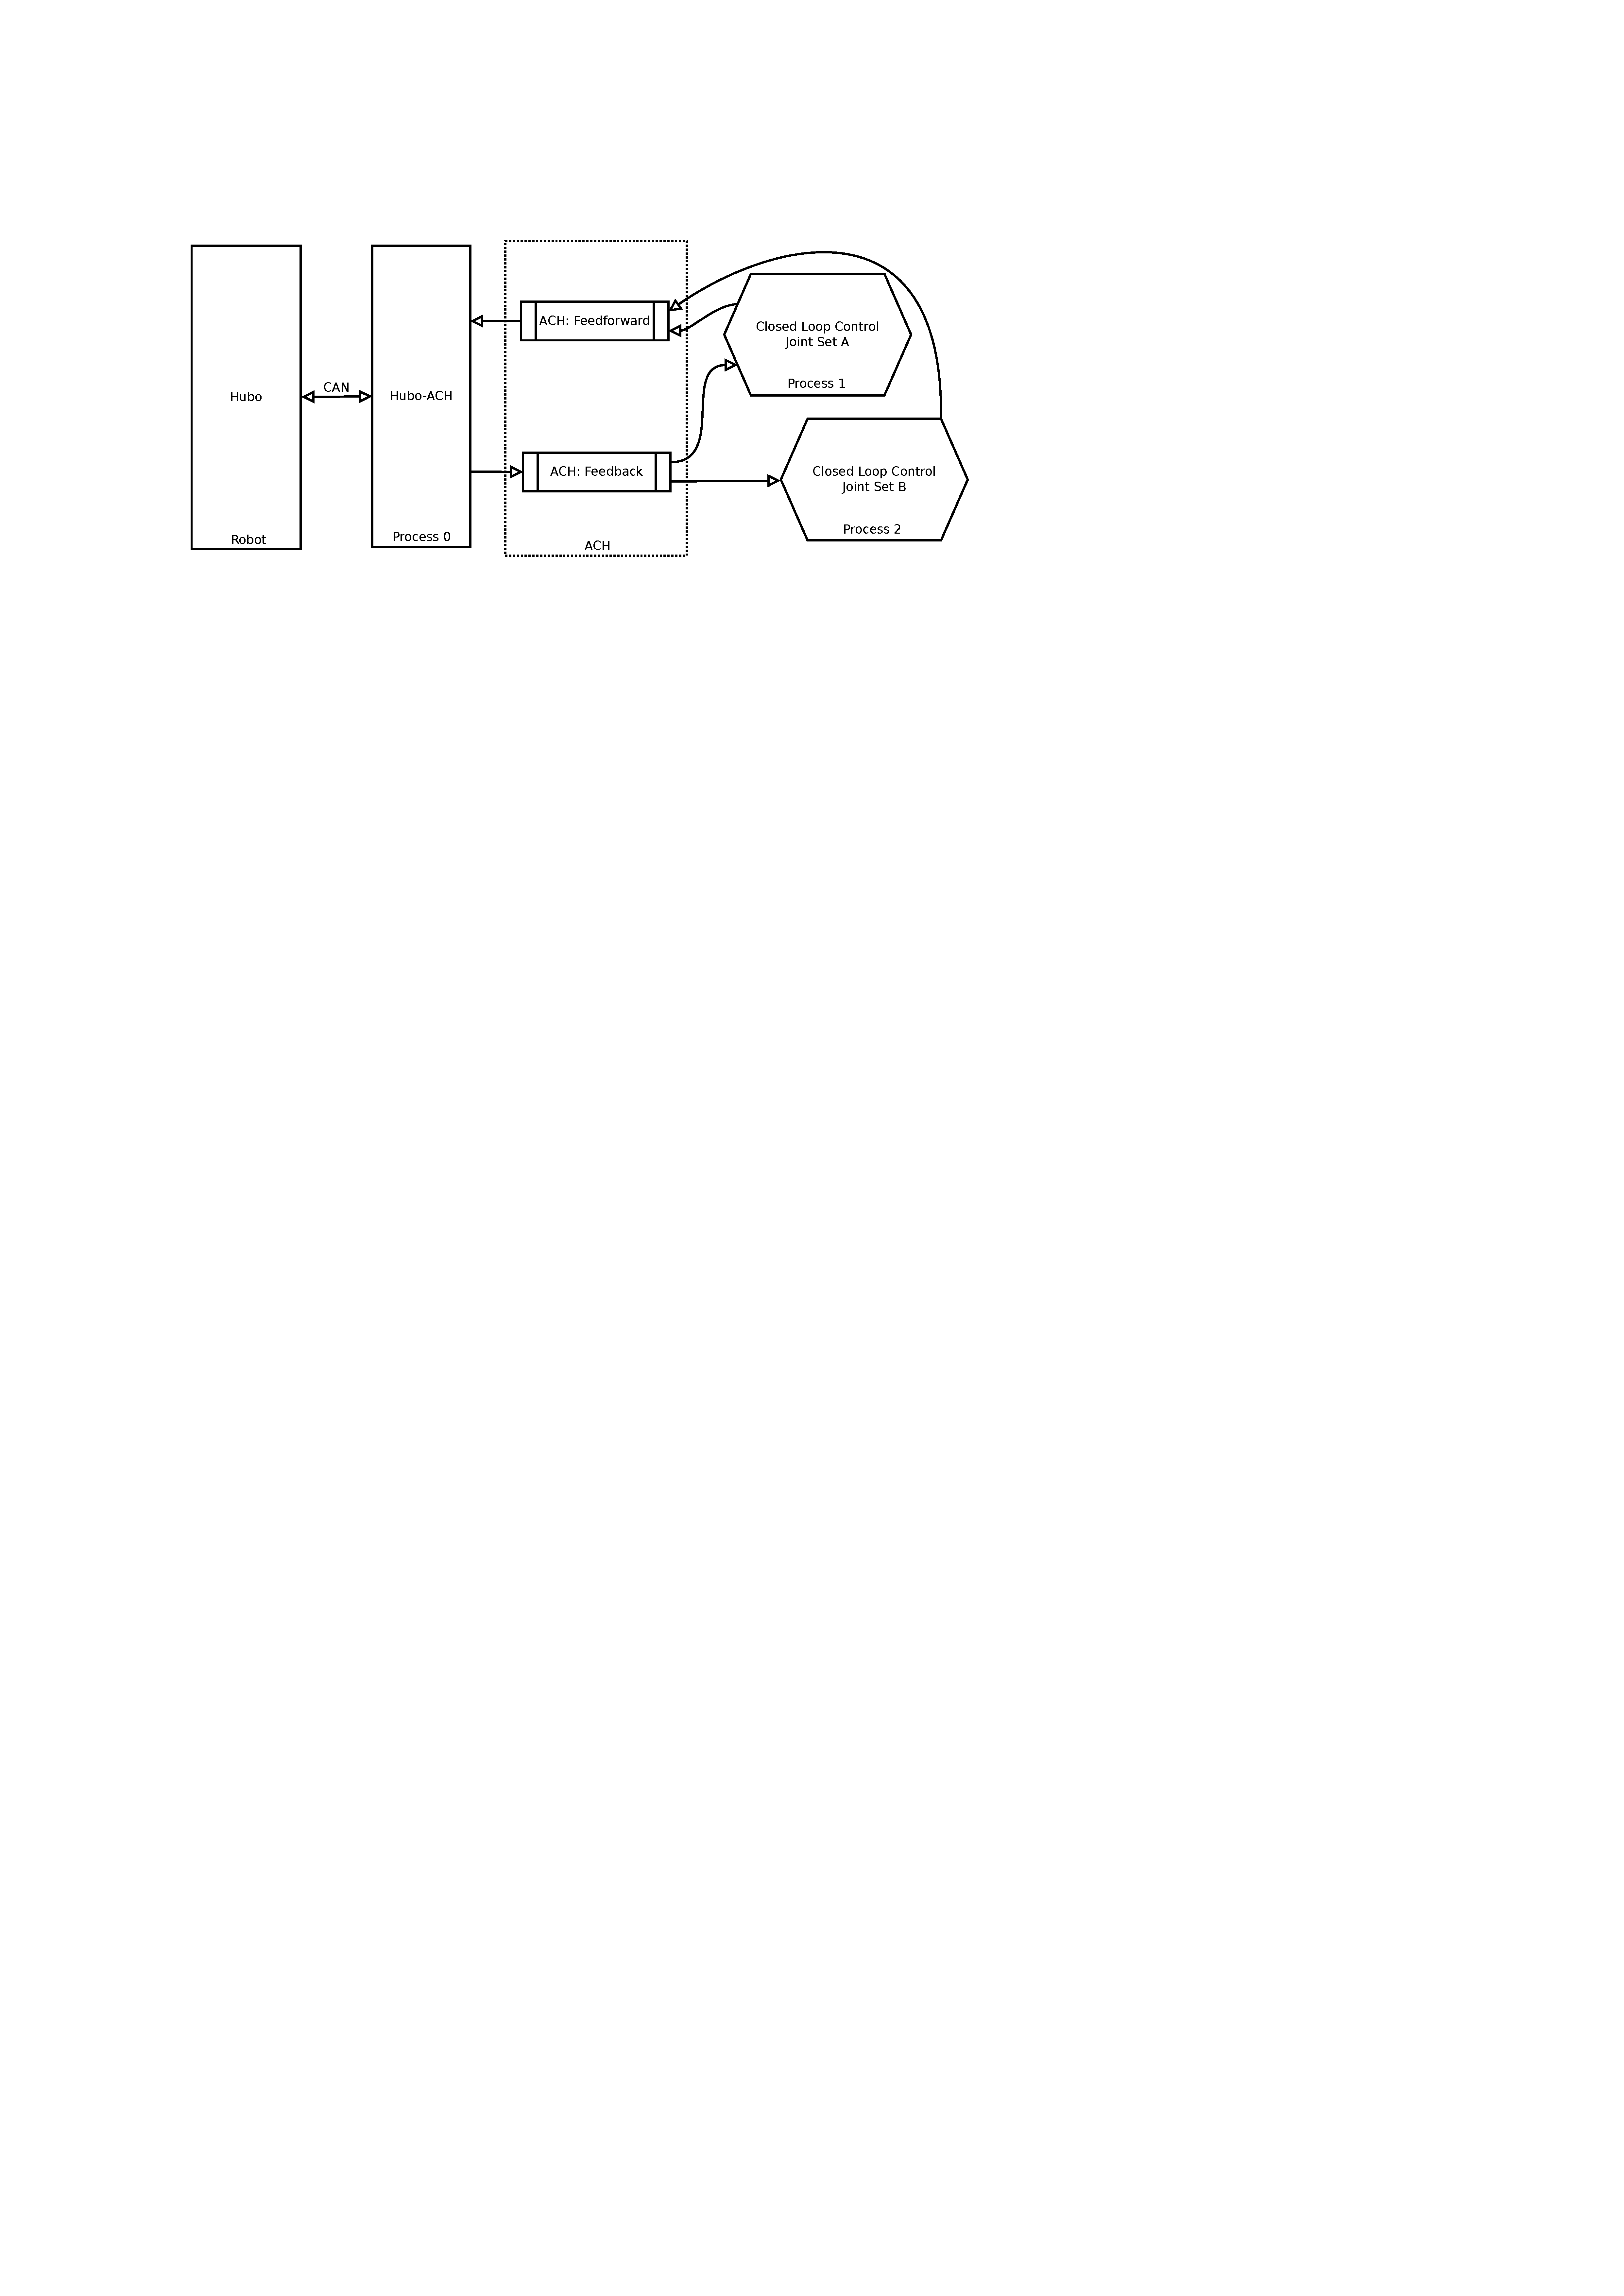
\includegraphics[width=1.0\columnwidth]{./pix/hubo-ach-diagram.pdf}
  \caption{Hubo Primary Controller (HPC) and system framework}
  \label{fig:graph}
\end{figure}





 Primary Hubo Controller (PHC) also known for the Hubo2 Plus full-size humanoid robots.  
The Hubo2 Plus is a 130 $cm$ tall humanoid robot commonly referred to as Hubo.  
Hubo weighs 37 $kg$ and has 40 DOF.
Each DOF, with the exception of the fingers, are high gain PD position controlled .  
There are 12 DOF in each leg, roll, pitch and yaw in the hip, pitch in the knee and roll and pitch in the ankle.  

The PHC runs on the concept of using separate process for 



The primary PHC process is a daemon that talks over the CAN bus to all of the Hubo motor drivers and sensors.  
The \textit{feedforward} and \textit{feedback} states are stored in the \textit{HUBO\_REF\_CHANNEL} and \textit{HUBO\_STATE\_CHANNEL}.  
All information is stored in SI units.  The \textit{HUBO\_REF\_CHANNEL} holds a strut that has the desired reference for each of the joints in $rad$.  
The \textit{HUBO\_STATE\_CHANNEL} contains the sensor data and that joint status data.  
This includes:

\begin{itemize}
                \item Encoder position (rad), at each joint
                \item IMU x angle (rad), at CoM
                \item IMU y angle (rad), at CoM
                \item IMU Vx velos(rad/sec), at CoM
                \item IMU Vy velos(rad/sec), at CoM
                \item FT Mx moment (Nm), in Feet
                \item FT My moment (Nm), in Feet
                \item FT Fz force (N), in Feet
                \item Angle from acc Ax (rad), in Feet
                \item Angle from acc Ay (rad), in Feet
                \item G-force acc Az (G), in Feet
\end{itemize}

The PHC daemon runs in real-time using the preempt-rt kernel.  
All sensors are polled and motor references are set at the system period.  
This period is currently set to 0.004 $sec$, $T_H$.  
This period is limited by the bandwidth of the CAN communications bus which is currently set to 1.0 $Mbps$.  
Currently there are two CAN channels with one controlling the upper body and one the lower body.  
The operation frequency can be increase if more CAN channels are added.  
The PHC system is designed for ease of adding communication busses.  

At the beginning of each cycle the new references are set to each actuator.  
After each cycle the state is updated with the new sensor data.

A separate process will subscribe to the \textit{feedforward} and \textit{feedback} channels and run it's own real-time loop.  
This can run, update reference and read the feedback channel at any desired frequency within the processor and IPCs capabilities.
The PHC will always take the most recent reference from the feedforward channel at the rising edge of it's clock cycle with the period of $T_H$.
This ensures the motor drivers are updated at a constant rate. 
Each motor driver accepts a position reference and uses a phase locked loop (PLL) to lock onto the frequency and timing of the incoming reference commands.
The motor driver then linearly interpolates the reference commands from the current position to the set position to increase the commanded rate to the motor itself by 5 times the command frequency, $\frac{1}{T_H}$.
This is done to reduce the jerk of each of the actuated joints.

The key point is that the PHC runs with a period of $T_H$ and updates the motors with the references from the feedforward channel no matter what rate the external controller is updating the feedforward channel at.  
The sensors are also updated at a period of $T_H$.
The structure of the system can be found in Fig.~\ref{fig:graph}.

\begin{figure}[thpb]
  \centering
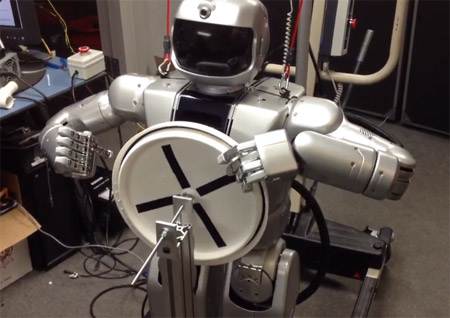
\includegraphics[width=1.0\columnwidth]{./pix/hubo_valve.png}
  \caption{Hubo running PHC turning a valve using trajectories created using Bi-RRTs. }
  \label{fig:valve}
\end{figure}

Current capabilities of the PHC system includes:

\begin{itemize}
\item Full Hubo2 Plus compatibility 
\item ROS support
\item Independent process for controllers
\item OpenRAVE trajectory playback
\item OpenHUBO integration 
\item Low frequency joint update filter.
\end{itemize}




